%==============================================================================
% Homework X, MATH-GA 2046 (Fall 2021)
%==============================================================================
\newcommand{\thisclass}{\bf MATH-GA 2046 }
\newcommand{\thishw}{\bf HW 1: Programming Portion}
\newcommand{\myname}{Oliver Hare}
\newcommand{\mylogin}{oph206}
\newcommand{\mygithub}{https://github.com/Buggy-Virus/SI-ML-Homework}

%==============================================================================
% Formatting parameters.
%==============================================================================

\documentclass[11pt]{article} % 10pt article, want AMS fonts.
\makeatletter					% Make '@' accessible.
\pagestyle{myheadings}				% We do our own page headers.
\def\@oddhead{\bf \thisclass - \thishw\hfill \myname (\mylogin)}
%\newline \today\hfill \mygithub} % Here they are.
\def\thesection{Problem\hskip-1em\ }		% Section headlines.
\oddsidemargin=0in				% Left margin minus 1 inch.
\evensidemargin=0in				% Same for even-numbered pages.
\textwidth=6.5in				% Text width (8.5in - margins).
\topmargin=0in					% Top margin minus 1 inch.
\headsep=0.2in					% Distance from header to body.
\textheight=8in					% Body height (incl. footnotes)
\skip\footins=4ex				% Space above first footnote.
\hbadness=10000					% No "underfull hbox" messages.
\makeatother					% Make '@' special again.

%\usepackage{newalg}
\usepackage{amsmath,amsfonts,amssymb}
\usepackage{csvsimple}
\usepackage{latexsym}
\usepackage{enumitem}
\usepackage{mathtools}
\DeclarePairedDelimiter{\ceil}{\lceil}{\rceil}

%==============================================================================
% Macros.
%==============================================================================
\newcommand{\problem}[1]{\section{#1}}		% Problem.
\newcommand{\new}[1]{{\em #1\/}}		% New term (set in italics).
\newcommand{\set}[1]{\{#1\}}			% Set (as in \set{1,2,3})
\newcommand{\setof}[2]{\{\,{#1}|~{#2}\,\}}	% Set (as in \setof{x}{x > 0})
\newcommand{\C}{\mathbb{C}}	                % Complex numbers.
\newcommand{\N}{\mathbb{N}}                     % Positive integers.
\newcommand{\Q}{\mathbb{Q}}                     % Rationals.
\newcommand{\R}{\mathbb{R}}                     % Reals.
\newcommand{\Z}{\mathbb{Z}}                     % Integers.
\newcommand{\compl}[1]{\overline{#1}}		% Complement of ...

%==============================================================================
% Title.
%==============================================================================


\begin{document}
\centerline{\LARGE}
\centerline{\LARGE\thishw}
\vspace{2mm} \newline
\centerline{\small github.com/Buggy-Virus/SI-ML-Homework/tree/master/assignment-1}
\centerline{\small\today}

\problem{2}
% %%%%%%%%%%%%%%%%%%%  PROBLEM 1 %%%%%%%%%%%%%%%%%%%%%%%%
My program for problem 2 is generally structured into four different functions and a main function, I'll summarize them quickly here.
\begin{itemize}
    \item generate\_curve\_function \\
    This returns a callable function which is some polynomial with noise. The number of variables and degrees are passed, as well on parameters to control the random variables that are generated for coefficients and parameters to use as noise parameters every time the created function is called.
    \item create\_data \\
    Create data simply takes in the number of observations, predictions, and a callable function and creates a number of predictor vectors with the length of the number of observations, each vector is generated with a Gaussian function with different parameters for mean and noise for each predictor vector. These are stitched together to form $x$, and then the function is called on $x$ to get $y$.
    \item get\_curves \\
    Get curves does most of the heavy lifting. iterating through the number of instances we want to run (in this case 100). And each instance creating data for both training and testing (50 obs for each here), and then iterating from 0 to the max complexity (35 in this case), each time training a polynomial Lasso model using SKlearn with a degree equal to the current complexity. \newline
    This model then has its mean squared error for the predictor having been fed the training data. This represents the training error. Which we then take the mean of all the MSQE at each complexity to create a curve representing the expected test error. \newline
    Additionally at each of these complexities for each of these instances, an equally another $x$ as large as the training set, which was reserved from training is used for prediction, and compared against the real $y$ that was generated along with the data. This represents the conditional test error, and similarly it takes the mean across the complexities of these curves to get an estimate of the conditional test error.
    \item plot\_curves \\
    Plot curves does what it says, it plots the curves. I did have very high values for my error, so I took the log before plotting, which is why the mean curves do not look like they sit exactly in the middle of the curves they were generated from.
    \newpage

    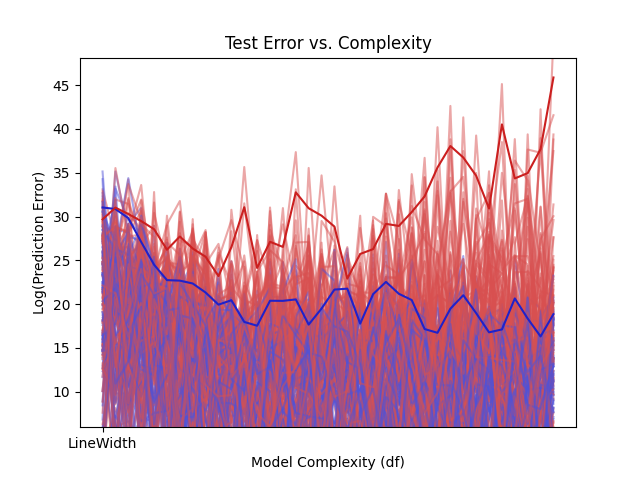
\includegraphics[scale=0.75]{slide_pic_recreation.png}

    Above you can see the result of the program. Which illustrates the point made in the original image that as complexity increases and fit of the training set increases, eventually it causes wild overfit and causes the conditional test error to begin exploding. This was generated with using a 9 degree polynomial as the underlying function.

    Regrettably the way I setup my program made it difficult for me to extract a graph where the individual curves and the resulting mean curves weren't overwhelming noisy. I experimented with various values passed to my curve function generate and my create data generator, but wasn't able to find more pleasant values in time.

    The below table shows the values for Test and Conditional Test Error mean and standard deviation at 0 degrees of freedom and 35. And you see the expected effect of it reducing for both  in the test case, while exploding at 35 for the conditional test error. If more data was presented we would also see the effect the graph shows of the red curve dropping initially as complexity increases to match that of the funtion.

\begin{center}
\begin{tabular}{||c c c c c||}
 \hline
 df & TE u & CTE u & TE std & CTE std \\ [0.5ex]
 \hline\hline
 0 & 3.001889e+13  & 7.702568e+12 & 1.964344e+14 & 3.181605e+13 \\
 \hline
 35 & 1.546179e+08 & 8.351572e+19 & 1.240098e+09 & 8.308365e+20 \\
 \hline
\end{tabular}
\end{center}
% %%%%%%%%%%%%%%%%%%%  PROBLEM 1 %%%%%%%%%%%%%%%%%%%%%%%%
\newpage
\problem{3}
% %%%%%%%%%%%%%%%%%%%  PROBLEM 2 %%%%%%%%%%%%%%%%%%%%%%%%
\newline
\csvautotabular{lasso_res.csv}\newline

I'm up against the wire, and am rushing to submit (not that it's an excuse) so I have to apologize about not formatting the data. correctly where you could see theirs against mine side by side.\newline

I was not able to converge to the same beta as glmnet generally, and my overall deviance was not as low. That being said looking into their code, I am unsure they were calculating deviance in the exact same way so it may have had an impact on the different between the two.\newline

That being said, the directions of my steps, and the lambdas when the degrees of freedom increased were generally the same, showing that it was following a similar path, even if it were not the case that the beta it converged to was the same.\newline

I'll try to resubmit nice data. (Just making sure I get something in.)
% %%%%%%%%%%%%%%%%%%%  PROBLEM 2 %%%%%%%%%%%%%%%%%%%%%%%%
\end{document}
